\section{Testing Runge-Kutta and Velocity-Verlet for Sun-Earth-Mars System}
\label{sec:SunEarthMarsTest}

Before using the codes to calculate the movement of the stars in a star cluster, the codes are tested on a known system like the Sun-Earth-Mars system. This is because these bodies move in a very predictable and stable fashion. So when increasing the time the orbits should remain almost equal to the initial orbit, and almost circular. As it is  possible to see in \figref{fig:SunEarthMarsTest} that it's the case. Where the mass, initial position and, velocity is set as given in \tabref{tab:SunEarthMarsTest}. 

\begin{table}[H]
\centering
\caption{Mass, initial position and initial velocity of Sun, Earth and Mars when running the Runge-Kutta 4 algorithm for this three-body problem.
The Earth and Mars are set to orbit in the $x-y$-plane at $z=1$ AU with the distance 1 AU and 1.5 AU to the Sun, respectively, which is not physically true. However, this initialization of position and velocity is reasonable to illustrate the validity of the Runge-Kutta method and Velocity-Verlet method presented in \secref{Newton2body3D}.
}
\begin{center}
\begin{tabular}{ | c | c | c | c |  }
  \hline			
   & mass [$M_{\odot}$] &  $\v{r}_{initial}$ [AU] & $\v{v}_{initial}$ [AU/day]  
  \\ \hline
  Sun & $1.0$ & $(1.0,1.0,1.0)$  & $(0.0,0.0,0.0)$ 
  \\ \hline
  Earth & $3.0\times 10^{-6}$ & $(2.0,1.0,1.0)$ & $(0.0,0.017,0.0)$
  \\ \hline
  Mars & $3.2\times 10^{-7}$ & $(-0.5,1.0,1.0)$  & $(0.0,0.014,0.0)$
  \\ \hline
\end{tabular}
\end{center}
\label{tab:SunEarthMarsTest}
\end{table}

    
\begin{figure}[H]
\centering
\begin{minipage}{.5\textwidth}
  \centering
  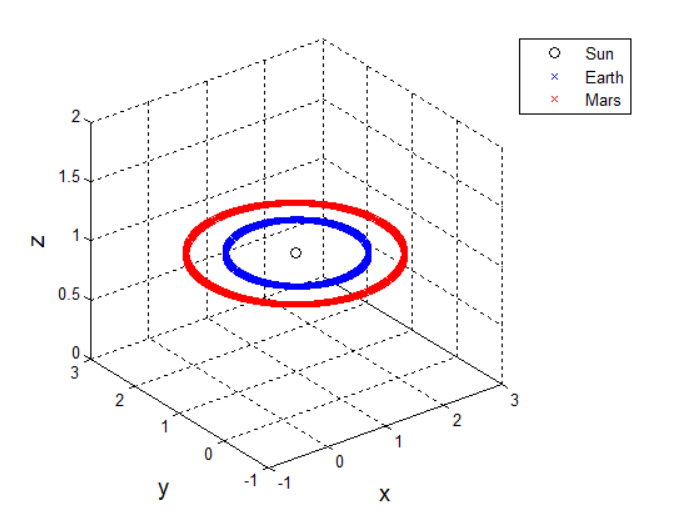
\includegraphics[width=1\linewidth]{Figures/sun_earth_mars_test_RK4.png}
\end{minipage}%
\begin{minipage}{.5\textwidth}
  \centering
  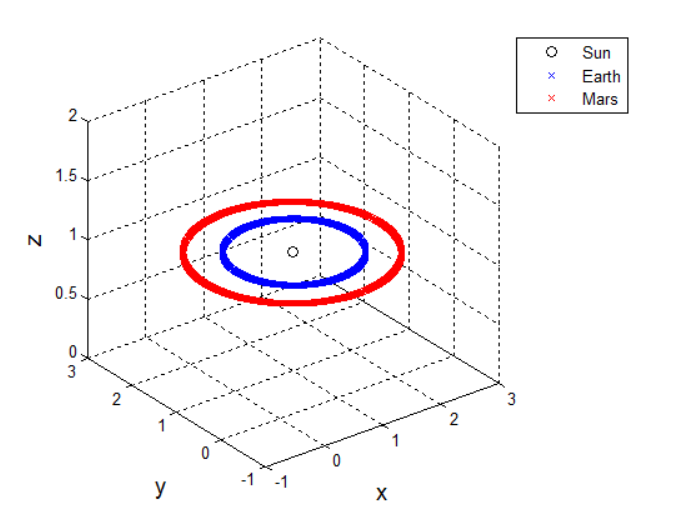
\includegraphics[width=1\linewidth]{Figures/sun_earth_mars_test_VV.png}
\end{minipage}
\caption{
Time evolution of the simplified system of Sun-Earth-Mars over a time period of 20 years using Runge-Kutta (leftmost) and Velocity-Verlet (rightmost) method with a time step length of 1 day.
The masses, initial positions, and initial velocities of the three objects are given in \tabref{tab:SunEarthMarsTest}.
}
\label{fig:SunEarthMarsTest}
\end{figure}

Calculating the initial and final energy of the Sun-Earth-Mars system according to the source code presented in \secref{sec:ComputingEnergy}, gives the \tabref{tab:SunEarthMarsTest_energy_conservation} for different time periods with step length of 1 day.

\begin{table}[H]
\centering
\caption{The final energy after different time periods computed by both the first order Runge-Kutta method and the Velocity-Verlet method for the Sun-Earth-Mars-like system with initial energy of $2.37\times 10^{-9} \text{M}_{\odot} \text{AU}^2 /\text{days}^2$ .
}
\begin{center}
\begin{tabular}{ | c | c | c |  }
  \hline	
  Time period (years) & Final energy (RK4) & Final energy (VV)
  \\ \hline		
  1  & $-1.44\times 10^{-9}$ & $-1.44\times 10^{-9}$
  \\ \hline
  10  & $-1.47\times 10^{-9}$ & $-1.47\times 10^{-9}$
  \\ \hline
  100  & $-1.48\times 10^{-9}$ & $-1.48\times 10^{-9}$
  \\ \hline
  1000 & $-1.44\times 10^{-9}$  & $-1.44\times 10^{-9}$ 
  \\ \hline
\end{tabular}
\end{center}
\label{tab:SunEarthMarsTest_energy_conservation}
\end{table}


From the results in \tabref{tab:SunEarthMarsTest_energy_conservation} the energy is not changing much over time, and with the precision of the constants, e.g. the gravitational constant $G=2.96\times 10^{-4} \text{AU}^3 / \text{days}^2 \cdot \text{M}_{\odot}$, and the time steps, this gives a good picture of the evolution of the energy. And it gives the impression that the methods used are giving a good estimates to the real movement of the particles. And since it is working for this model with three particles it is possible to assume that it will work for N bodies as well. 